\documentclass[tikz,border=10pt]{standalone}

% Hypergraph reconstruction with additive (induced subgraph) queries.
% Query set S contains hyperedges e1, e2 fully; e3 crosses the boundary.
% Oracle answer: 2.

\usepackage{tikz}
\usetikzlibrary{arrows.meta,calc,backgrounds}
\usepackage{amsmath,amssymb}
\usepackage{xcolor}

\definecolor{e1color}{RGB}{0,100,200}
\definecolor{e2color}{RGB}{0,140,60}
\definecolor{e3color}{RGB}{200,50,50}
\definecolor{querycolor}{RGB}{150,50,150}

\begin{document}
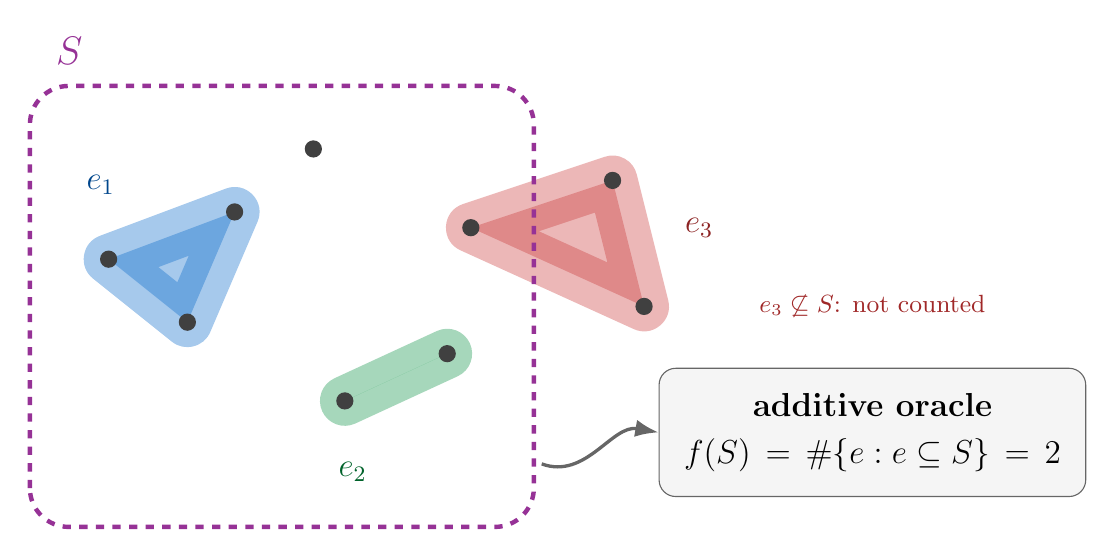
\begin{tikzpicture}[
  vtx/.style={circle, fill=black!75, inner sep=2.2pt},
  vlabel/.style={font=\small},
  blob/.style={line width=18pt, line cap=round, line join=round, draw opacity=0.35, fill opacity=0.35},
]

% ---------- vertices ----------
\node[vtx] (v1) at (0.0, 2.2) {};
\node[vtx] (v2) at (1.6, 2.8) {};
\node[vtx] (v3) at (1.0, 1.4) {};
\node[vtx] (v4) at (3.0, 0.4) {};
\node[vtx] (v5) at (4.3, 1.0) {};
\node[vtx] (v6) at (4.6, 2.6) {};
\node[vtx] (v7) at (6.4, 3.2) {};
\node[vtx] (v8) at (6.8, 1.6) {};
\node[vtx] (v9) at (2.6, 3.6) {};

% ---------- hyperedges as blobs ----------
\begin{scope}[on background layer]
  \draw[blob, e1color, fill=e1color] (v1.center) -- (v2.center) -- (v3.center) -- cycle;
  \draw[blob, e2color, fill=e2color] (v4.center) -- (v5.center);
  \draw[blob, e3color, fill=e3color] (v6.center) -- (v7.center) -- (v8.center) -- cycle;
\end{scope}

\node[e1color!70!black, font=\large] at (-0.1, 3.15) {$e_1$};
\node[e2color!70!black, font=\large] at (3.1, -0.5) {$e_2$};
\node[e3color!70!black, font=\large] at (7.5, 2.6) {$e_3$};

% ---------- query set S ----------
\draw[querycolor, dashed, line width=1.6pt, rounded corners=14pt]
  (-1.0, -1.2) rectangle (5.4, 4.4);
\node[querycolor, font=\Large\bfseries] at (-0.5, 4.85) {$S$};

% ---------- oracle ----------
\node[draw=black!60, fill=black!4, rounded corners=6pt, align=center,
      font=\large, inner sep=9pt] (oracle) at (9.7, 0.0)
  {\textbf{additive oracle}\\[3pt]
   $f(S) \,=\, \#\{e : e \subseteq S\} \,=\, 2$};
\draw[-Latex, very thick, black!60] (5.5, -0.4) to[out=-20, in=170] (oracle.west);

% note: e3 crosses the boundary, not counted
\node[e3color!80!black, font=\small, align=center] at (9.7, 1.6)
  {$e_3 \not\subseteq S$: not counted};

\end{tikzpicture}
\end{document}
